\documentclass{beamer}
\usetheme{owl}           % Use metropolis theme
\title{Quantifying and Mimicking Networked Behavior in Social Insects}
\date{\today}
\author{Lucas Saldyt}
\institute{Arizona State University}

\begin{document}
  \maketitle
  %% \begin{frame}{Biomimicry of Distributed Behavior in Social Insects}
  %%     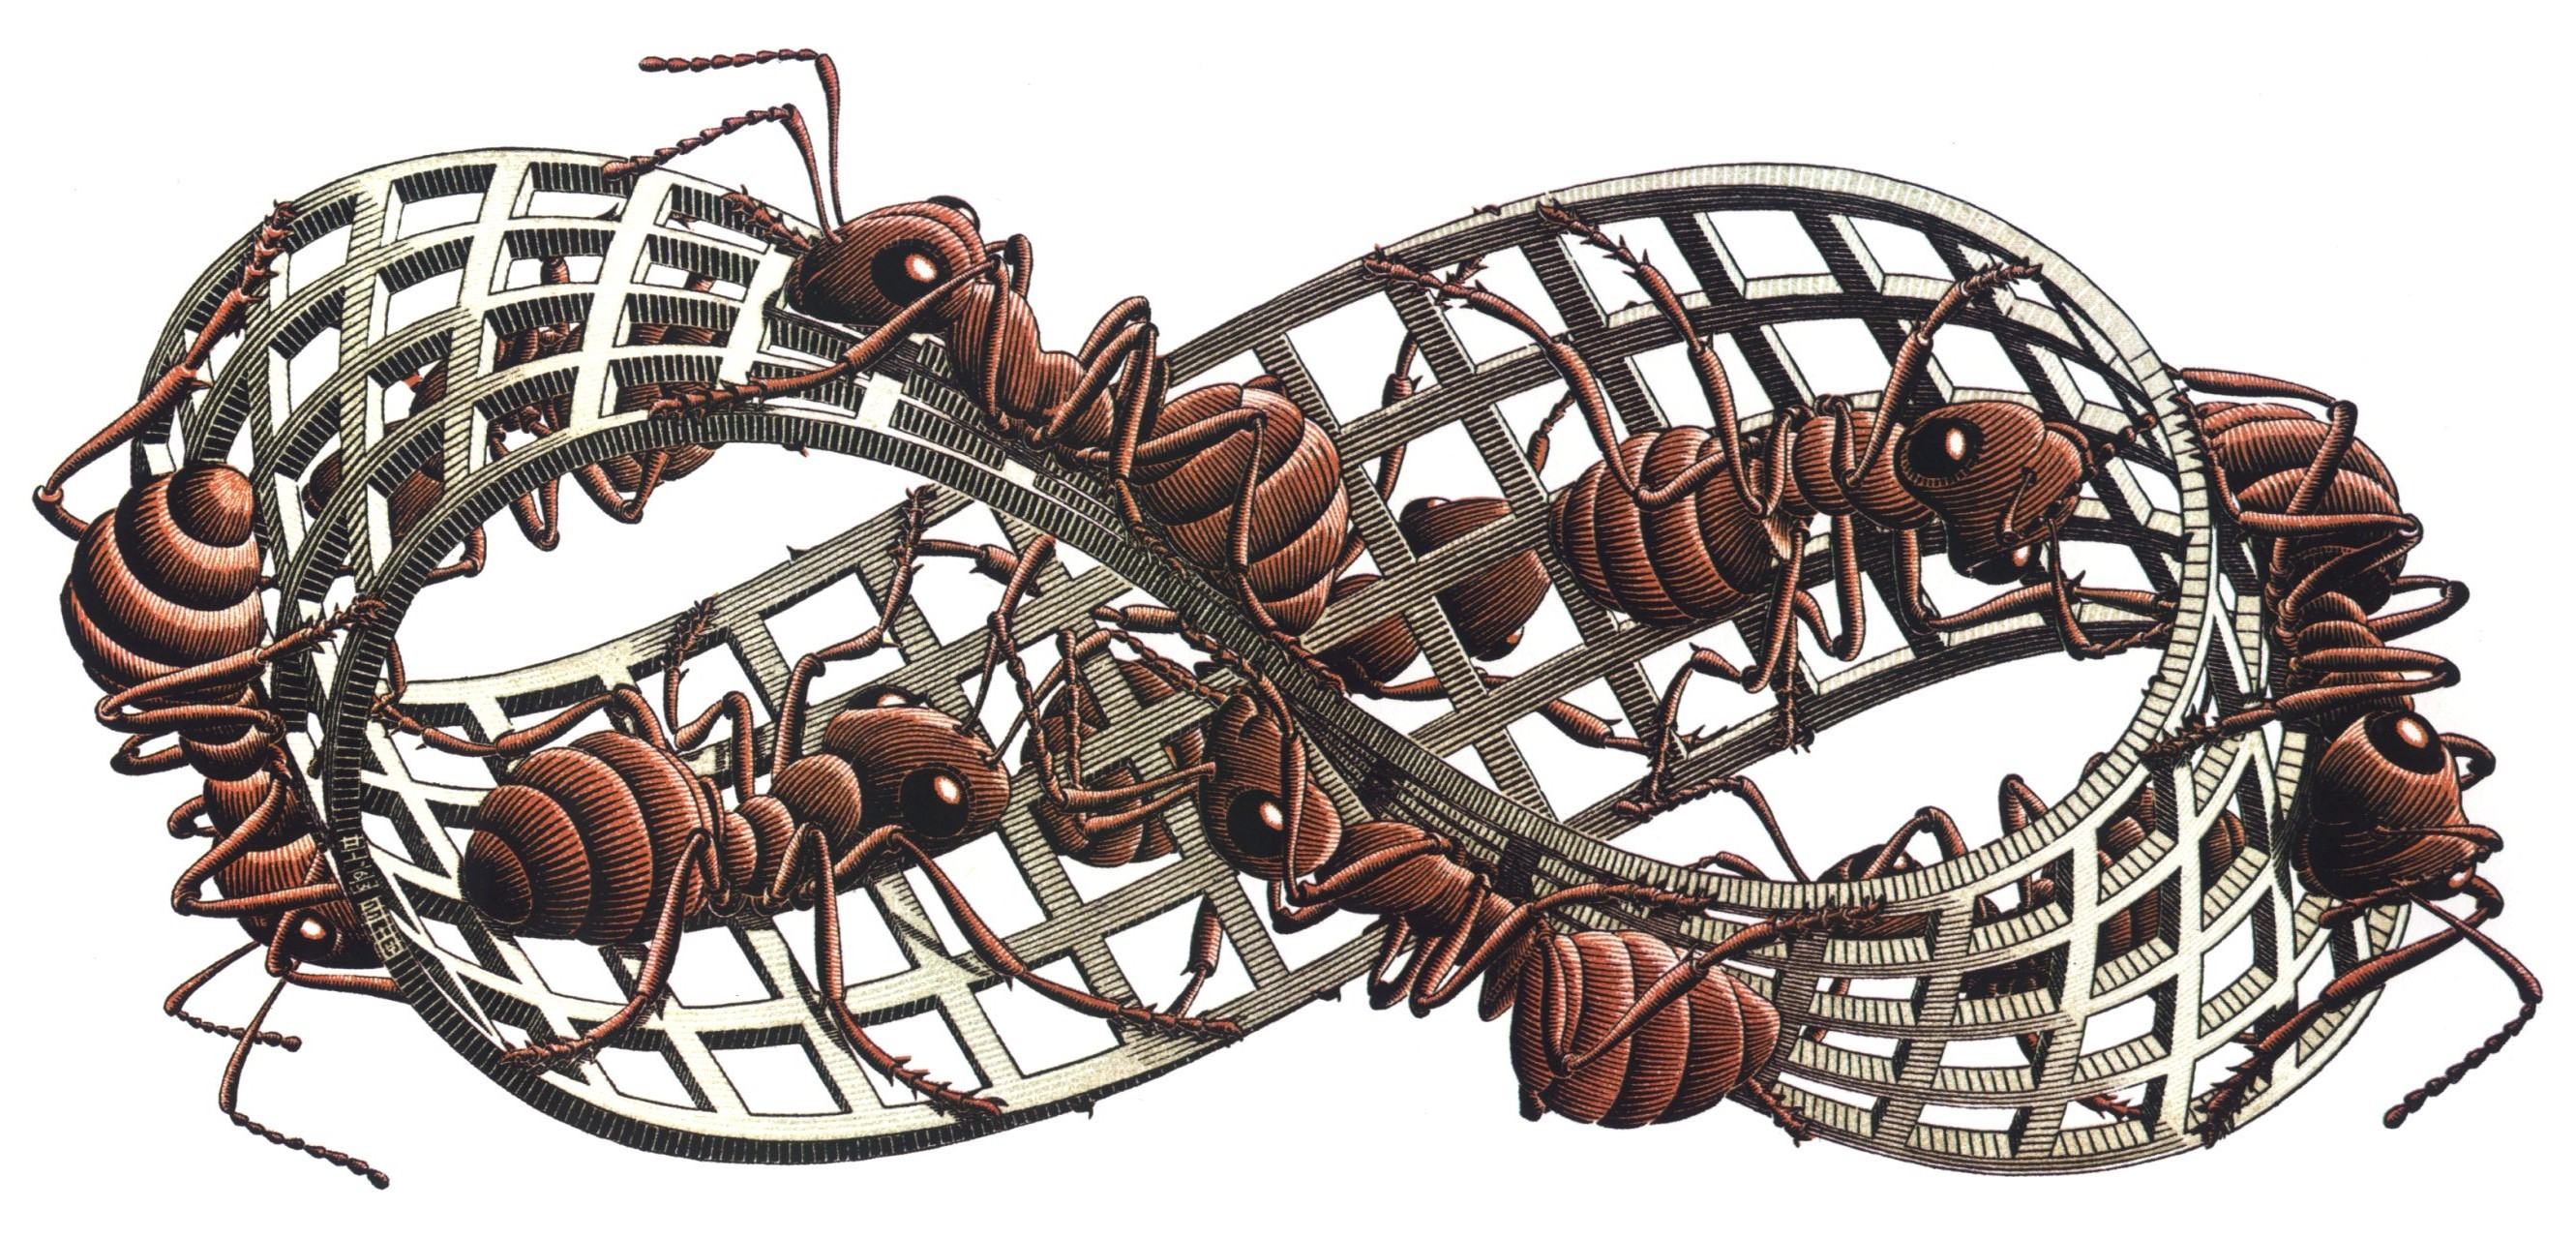
\includegraphics[scale=0.1]{ants}
  %% \end{frame}
  \begin{frame}{Scope and Motivation}
      \begin{itemize}
          \item Efficient Bottom-Up Self Organization
          \item Dynamic Self-Conditioned Response Behavior
          \item Generalizable Dynamics \tiny (See Applications) \\
      \end{itemize}
      %% Guntai Ali
  \end{frame}

  \begin{frame}{Applications In Order of Increasing Interest}
      \begin{itemize}
          \item Behavior in other social insects
          \item Biomimetic algorithms (i.e. Pathfinding)
          \item Swarm robotics (Construction, Defense)
          \item Efficient distributed simulation
          \item Social network dynamics (Idea spread)
          \item Agent based cognitive architectures
      \end{itemize}
  \end{frame}

  \begin{frame}{Individuals}
      \begin{itemize}
          \item Solitary Insects have developed for millions of years.
          \item Individual ant brains have ~15,000 neurons. (Compare to C Elegans). \newline
              \tiny (And neurons themselves are non-linear systems, so an ant colony has at least three levels of non-linearity: colony, brain, and neuron). \normalsize
          \item On their own, insects are already capable of non-trivial tasks (like pathfinding)
      \end{itemize}
  \end{frame}

  \begin{frame}{Eusociality}
      \begin{itemize}
          \item Insects fill separate roles with a high degree of cooperation \tiny (Ants are perfect communists?) \normalsize
          \item Colony-level behavior comes from communication. Ants use pheromone systems and touch-communication.
              \begin{itemize}
                  \item Ants can convey simple alarm responses, but also more complicated information, like paths.
              \end{itemize}
          \item High connectivity (possibility for rapid spreading)
          \item ``Stigmergy`` (Next Slide)
      \end{itemize}
  \end{frame}

  \begin{frame}{Stigmergy}
      ``Stigmergy is a form of self-organization social network. It produces complex, seemingly intelligent structures, without need for any planning, control, or even direct communication between the agents. As such it supports efficient collaboration between extremely simple agents, who lack any memory, intelligence or even individual awareness of each other`` - Wikipedia (Itself a stigmergic system!)
  \end{frame} 

  \begin{frame}{Collective Cognition}
      \begin{itemize}
          \item Signals like alarm unconditioned
          \item Signals like trail finding double-checked \tiny (Allows escape of local minima!) \normalsize
          \item Stigmergic Construction of particular interest:
              \begin{itemize}
                  \item Building blocks initially placed ``randomly``, and infused with pheromones.
                  \item Secondary blocks placed based on other blocks and recency
                  \item Local rules become intricate nests
              \end{itemize}
      \end{itemize}
  \end{frame}

  \begin{frame}{Model}
      Simple model: random correlated walk, where proximity determines spreading activation.
      \begin{itemize}
          \item Individual paths/locations wont be maintained
          \item Are group statistics maintained? (Like clustering coefficient or average velocity)
      \end{itemize}
  \end{frame}

  \begin{frame}{Cognitive Architectures}
      \begin{itemize}
          \item First cognitive architecture in the 50s (Newell and Simon). Turned into SOAR.
          \item Copycat: agent based model of creative problem solving
          \item LIDA: Combined general cognitive psychology with Copycat architecture.
          \item Agent based approaches like copycat or lida are comparable to our agent based ant model.
          \item Both also are controlled by PDE.
          \item For instance, copycat has equillibrium points and attractors -- some of them intentionally built in.
      \end{itemize}
  \end{frame}
  %% \begin{frame}{Problem}
  %%     Ant colonies are capable of rudimentary problem solving.
  %%     Problem solving in ant colonies is fundamentally different than classical conceptions of problem solving.
  %%     Ant colonies act as a distributed but dense network of independent agents.
  %%     At times, the colony can act independently.
  %%     At other times, the colony cooperates as a whole.
  %%     This emergence of organization is extremely interesting:
  %%     How does the signal propogate?
  %%     When does it propogate?
  %%     Is this method of co-operation more useful? Why/Why not?
  %% \end{frame}

  %% \begin{frame}{Using Columns}
  %%     \begin{columns}
  %%     \column{0.5\textwidth}
  %%     Left
  %%     \column{0.5\textwidth}
  %%     Right
  %%     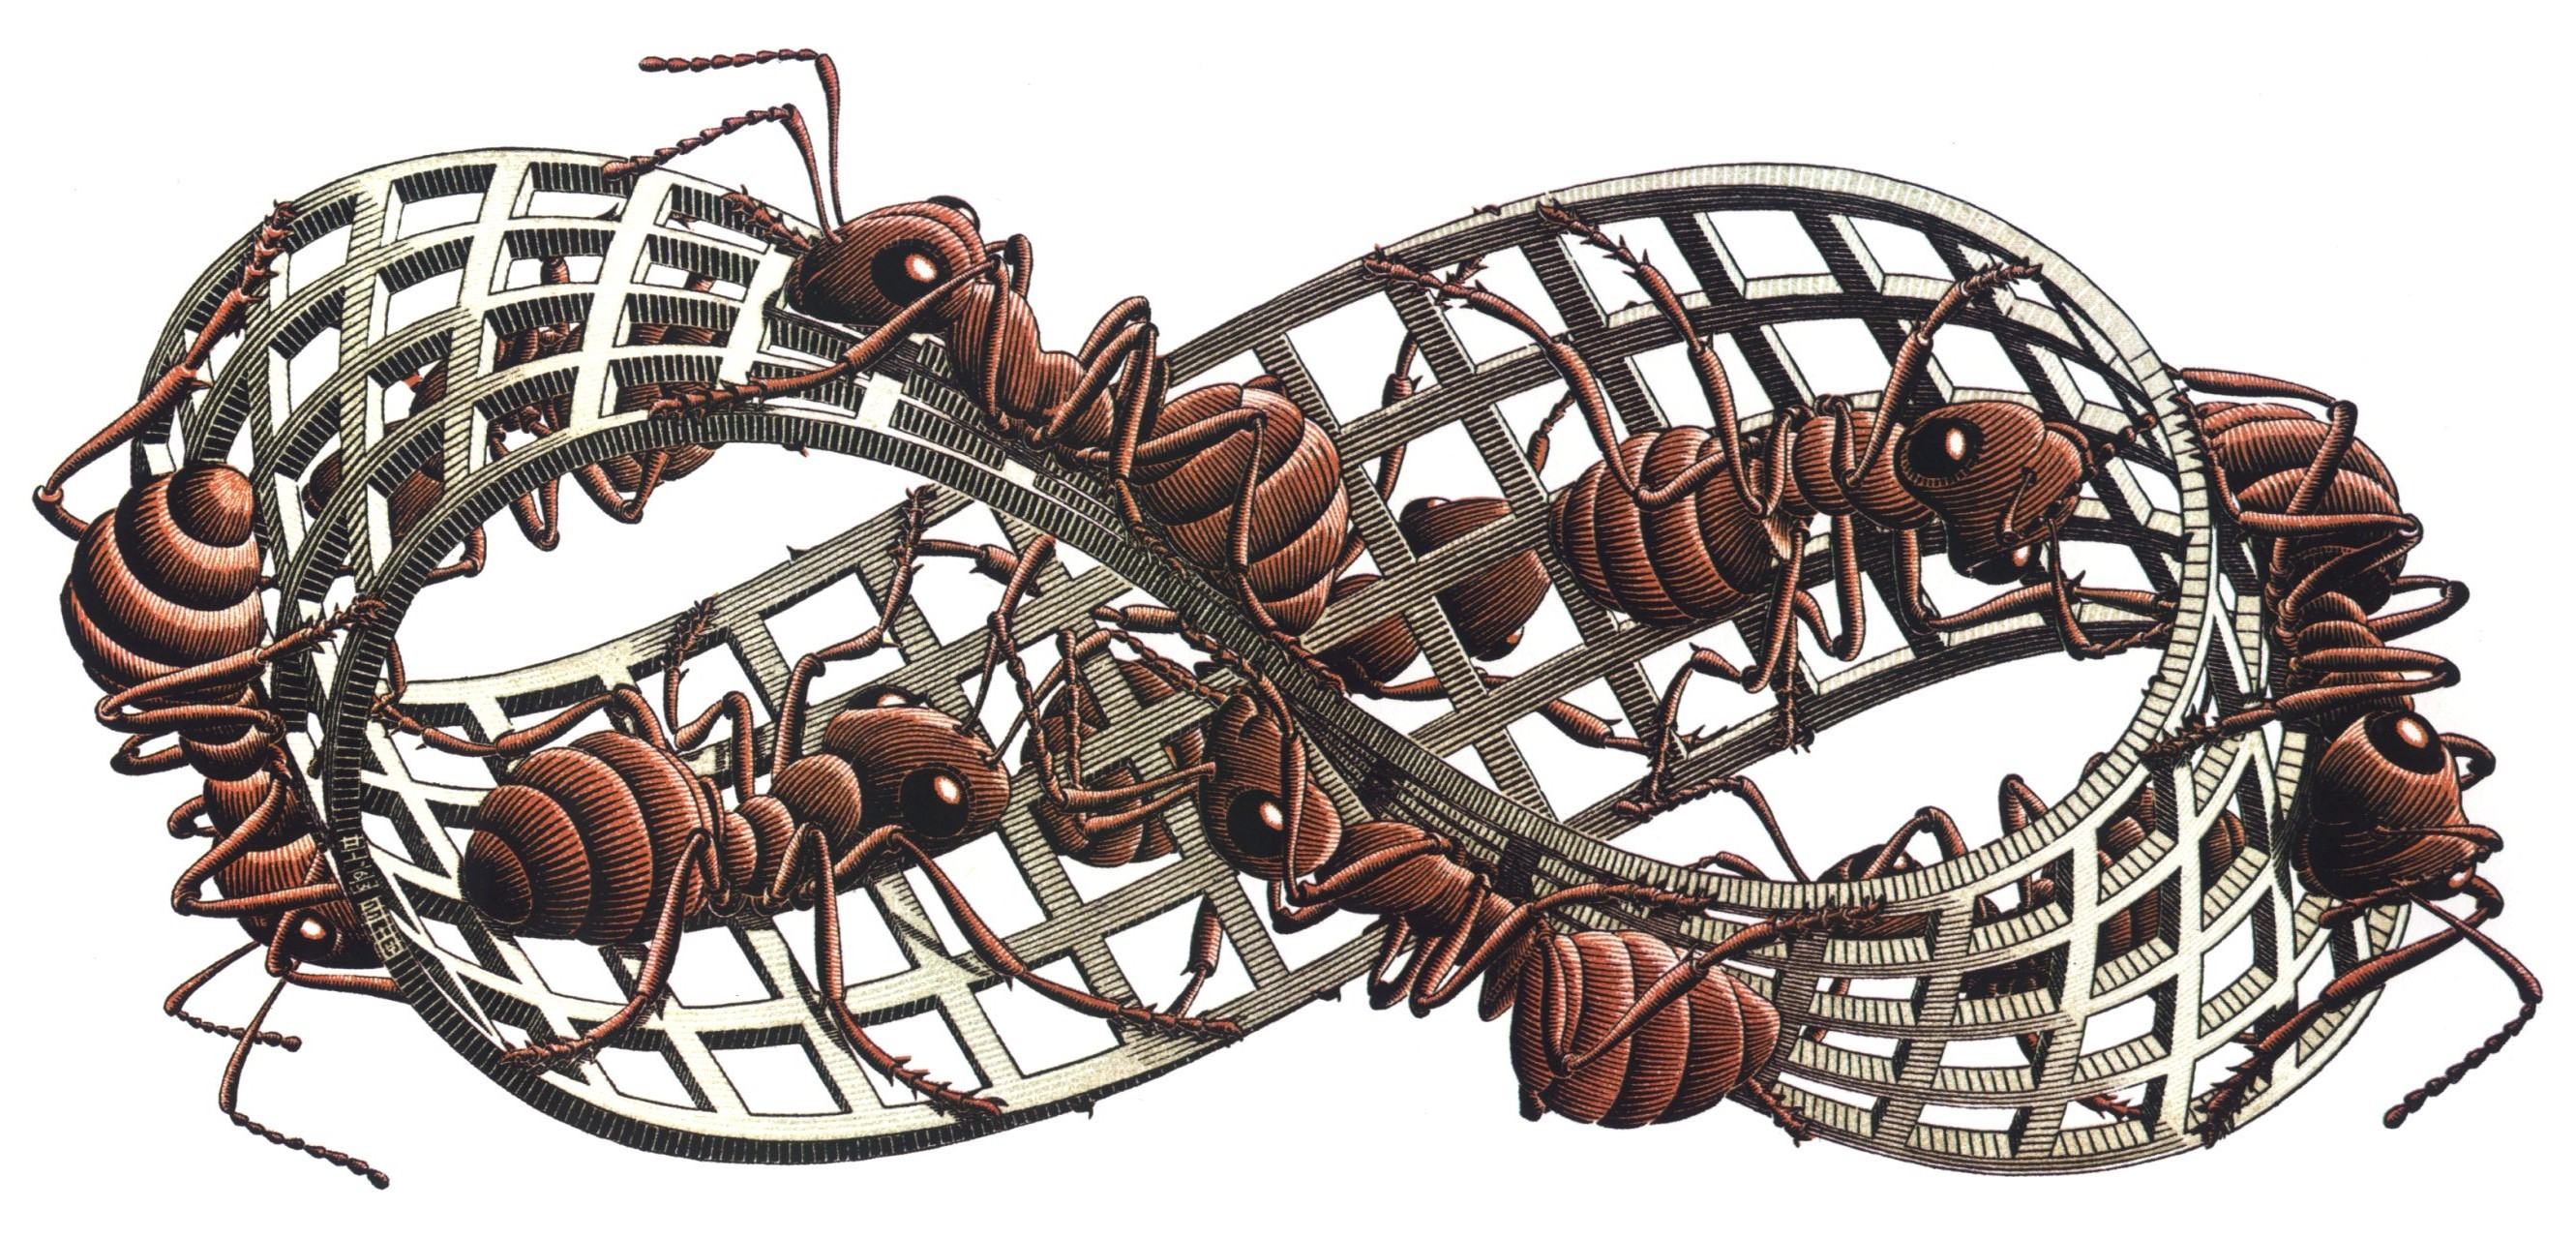
\includegraphics[scale=0.05]{ants}
  %%     \end{columns}
  %% \end{frame}
  %% \begin{frame}{Motivation}
  %%     Properties of ant colonies are likely present in other systems
  %%     Success has been had in designing algorithms based on the analogy of an ant colony
  %%     Networks in general are everpresent in todays society
  %%     (Networks are one of the most general data structures: understanding them is crucial)
  %% \end{frame}

  %% \begin{frame}{History}
  %%     Ant systems have been successfully studied in the past, and used to write computer algorithms.
  %%     %% In general, everything is biomimicry.
  %%     A certain class of cognitive architectures acts much like an ant colony
  %%     codelets = ants
  %%     castes = codelet types
  %%     workspace, other structures = colony components and environment
  %%     Specifically

  %%     Let us focus on the method by which ants construct their colonies, distributedly.
  %%     %% Ants are capable of doing so without using a blueprint by [ ](research).
  %%     This is of particular interest because of the idea of generative grammars.
  %%     %% Given [] pieces, build [] that does [].
  %% \end{frame}

  %% \begin{frame}{Levels}
  %%     Ants themselves have brains..
  %%     Which are themselves nonlinear
  %%     And the neurons in their brains.. are also nonlinear..
  %%     So: composition and emergence? What's interesting here?
  %%     Is it ever appropriate to assume that a level can be approximated linearly? 
  %%     %% (Are there hofstadterian symbolic layers?)
  %%     How close can an ant-model approximate the behavior of an ant colony?
  %%     Is it completely necessary to model everything (say, down to the level of quarks!?)
  %%     Micro vs Macro predictions and inevitability: like an ideal gas.
  %%     Even if we can't predict the locations and velocities of individual ants, we can still predict other factors, especially if they are statistically derived summary factors (like a metric quantifying alertness)
  %% \end{frame}

  %% \begin{frame}{Applications}
  %%     Anything related to network propogation.
  %%     Social media info spreading vs ant colony info spreading?
  %%     See: Carlos Castillo Chavez and the spreading of feynman diagrams.

  %% \end{frame}

  \begin{frame}{Definitions}
      This project focuses on the temporal network of ants.
      Ants are observed by a 30hz camera.
      Therefore, these observations are discrete.
      At each timestep, we know the network of ants. 
      We model this as a graph, with edges drawn as euclidean distances between each ant.
      While it is extremely difficult to create a model that maintains ant location and velocity, we hope to create a model that can produce the same network metrics and averaged behavior.
      Given the graph, we can calculate, for example, the way that the clustering coefficient changes over time.
  \end{frame}
\end{document}
